% ============================================================
%  深圳大学实验报告（SZU Experiment Report Template）
%  This template can be modified according to the specific requirements of your experiment or project.
%  Produced by: Chao Fan and Kewei Ou, AI School of SZU
% ============================================================

\documentclass[a4paper,11pt]{article}

% ----------------------------
% 中文与字体支持
% ----------------------------
\usepackage{fontspec}
\usepackage{xeCJK}
\setCJKmainfont{Noto Serif CJK SC}

% ----------------------------
% 页面设置与常用宏包
% ----------------------------
\usepackage{geometry}
\geometry{left=1in, right=1in, top=1in, bottom=1in}

\usepackage{amsmath,amssymb}
\usepackage{booktabs}
\usepackage{array}
\usepackage{longtable}
\usepackage{graphicx}
\usepackage{fancyhdr}
\usepackage{tikz}
\usetikzlibrary{calc}
\usepackage{verbatim}
\usepackage{float}
\usepackage{xcolor}
\usepackage{enumitem}
\usepackage{titlesec}
\usepackage[font=small,labelfont=bf,skip=4pt]{caption}
\usepackage[colorlinks=true,linkcolor=blue!70!black,urlcolor=blue!70!black,citecolor=blue!70!black]{hyperref}

\setlength{\parindent}{2em}
\setlength{\parskip}{2pt}
\linespread{1.15}
\titlespacing*{\section}{0pt}{8pt}{4pt}
\titlespacing*{\subsection}{0pt}{5pt}{2pt}
\setlist[itemize]{nosep, leftmargin=1.6em, topsep=2pt}
\setlist[enumerate]{nosep, leftmargin=1.8em, topsep=2pt}

\definecolor{myred}{RGB}{200,28,24}
\newcommand{\mywork}[1]{\textcolor{myred}{\textbf{#1}}}

% ----------------------------
% 页眉页脚设置
% ----------------------------
\fancyhf{}
\fancyhead[C]{}
\fancyhead[R]{}

\begin{document}

% ============================================================
% 封面页
% ============================================================
\begin{titlepage}
    \centering
    \vspace*{2cm}
    \Huge{\textbf{深 \ 圳 \ 大 \ 学 \ 实 \ 验  \ 报 \ 告}}\\[1.5cm]
    
    {\Large\textbf{课程名称}\quad\underline{\makebox[8cm][c]{Python程序设计}}}\\[0.5cm]
{\Large
\noindent\makebox[3.2cm][l]{\textbf{项目名称}}
\underline{\makebox[8cm][c]{ViT 图像编码器复现（NumPy）}}}\\[0.5cm]
{\Large
\noindent\makebox[3.2cm][l]{\textbf{学 \quad \quad 院}}
\underline{\makebox[8cm][c]{人工智能学院}}}\\[0.5cm]
{\Large
\noindent\makebox[3.2cm][l]{\textbf{专 \quad \quad 业}}
\underline{\makebox[8cm][c]{人工智能}}}\\[0.5cm]
{\Large
\noindent\makebox[3.2cm][l]{\textbf{指导教师}}
\underline{\makebox[8cm][c]{樊超}}}\\[0.5cm]
{\Large
\noindent\makebox[3.2cm][l]{\textbf{报 \quad 告 \quad 人}}
\underline{\makebox[3cm][c]{胡书奇}}
\hspace{0.5cm}
\textbf{学号}
\underline{\makebox[3cm][c]{2025040061}}}\\[0.5cm]
{\Large
\noindent\makebox[3.2cm][l]{\textbf{实验时间}}
\underline{\makebox[8cm][c]{2026年11月20日}}}\\[0.5cm]
{\Large
\noindent\makebox[3.2cm][l]{\textbf{提交时间}}
\underline{\makebox[8cm][c]{2026年11月23日}}}\\[1.5cm]

    \vfill
    \Large{\textbf{教务处制}}
\end{titlepage}

\newgeometry{left=0.9in, right=0.9in, top=0.82in, bottom=0.82in}

% ============================================================
% 正文部分
% ============================================================

\section{Objectives}

本次实验使用纯 NumPy（\texttt{float32} 精度）\mywork{复现 OpenCLIP ViT-B/32 图像编码器的前向推理过程}。给定预处理后的输入图像批次 $[B,3,224,224]$ 与 152 个模型权重张量，完成从图像切块、Token 嵌入、12 层 Transformer 编码到最终 512 维单位特征向量 $[B,512]$ 的计算，使各阶段输出与独立 FP32 参考结果在规定容差内保持一致，并保留与期末 Project 5（\texttt{szu\_python\_openclip}）兼容的模块接口。

\noindent\textbf{GitHub 代码仓库：}\href{https://github.com/bookie11/szu-python-project1-numpy}{https://github.com/bookie11/szu-python-project1-numpy}（包含 \texttt{image\_encoder.py}、\texttt{README.md} 与课前 NumPy 练习代码，大体积权重与参考数据未放入仓库）。

\section{Overview}

编码器整体计算流程如图~\ref{fig:vit-arch} 所示，左侧为主干数据流，右侧为单层 Pre-Norm \texttt{TransformerBlock} 的内部结构。图中蓝灰色部分为实验包已给出的预处理与基础算子（\texttt{PreprocessImage}、\texttt{LayerNorm}、\texttt{GELU}、\texttt{attention\_weights}、\texttt{unit\_vector}），\mywork{红色部分（\texttt{TODO-01} $\sim$ \texttt{TODO-06}）为我完成的核心代码}：
\begin{enumerate}
    \item[\mywork{Part 1}] \textbf{图像分块与嵌入（\mywork{TODO-01, TODO-05}）}：把 $[B,3,224,224]$ 切分为 $7\times 7=49$ 个展平块 $[B,49,3072]$，线性投影到 768 维后在最前面拼上 \texttt{CLS} 行并加上位置编码，得到 $[B,50,768]$；
    \item[\mywork{Part 2}] \textbf{多头注意力与残差网络（\mywork{TODO-02, TODO-03, TODO-04}）}：在 12 个 \texttt{TransformerBlock} 中把特征维拆成 12 个 64 维注意力头计算缩放点积注意力，结合两次残差相加与两层 MLP（中间层 3072 维）更新序列特征；
    \item[\mywork{Part 3}] \textbf{CLS 抽取与输出投影（\mywork{TODO-06}）}：取出第 0 个位置的 \texttt{CLS} 向量，做 \texttt{post\_norm} 和 $[768,512]$ 线性映射，再经单位化输出 $[B,512]$。
\end{enumerate}

\begin{figure}[H]
    \centering
    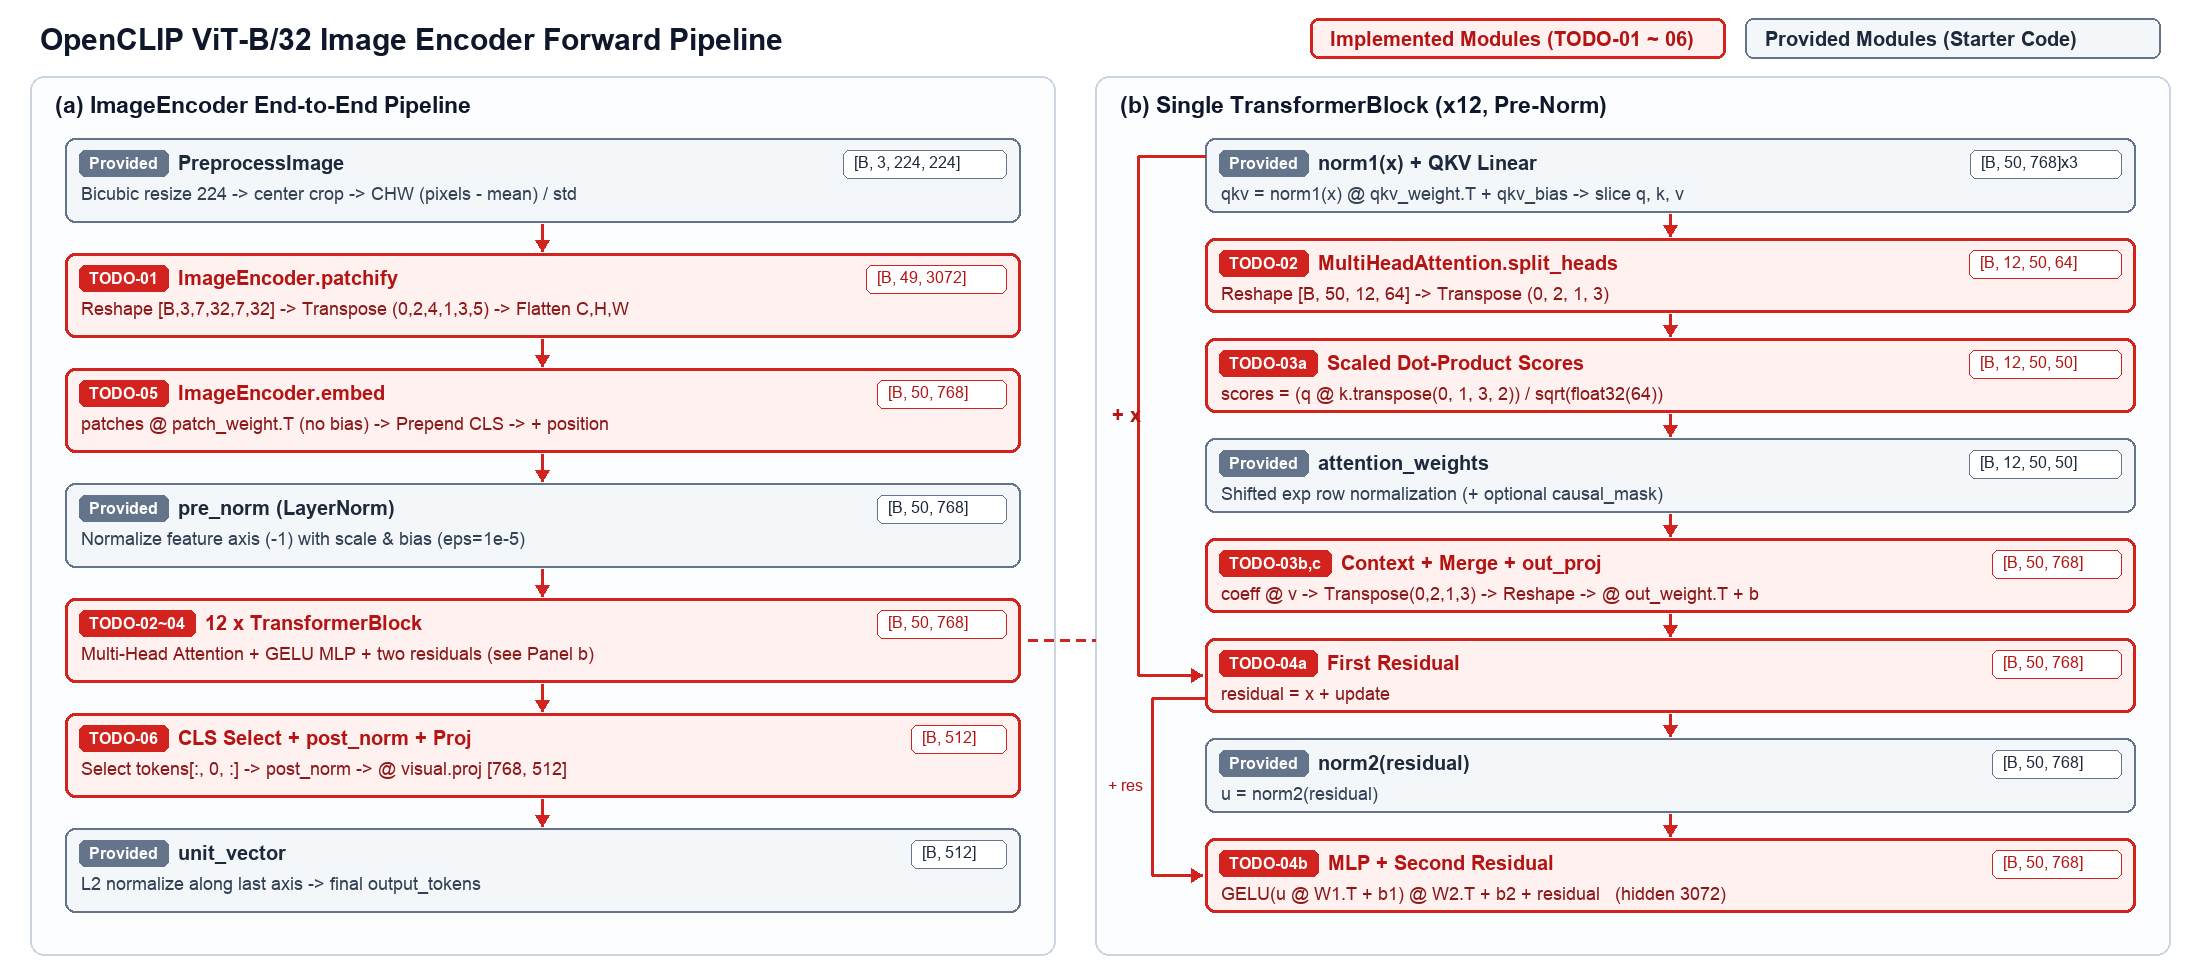
\includegraphics[width=0.98\linewidth]{figs/vit_overview.png}
    \caption{OpenCLIP ViT-B/32 图像编码器前向计算图。\mywork{红色框（TODO-01 $\sim$ TODO-06）为本人编写实现的模块}，蓝灰色框为已有辅助模块。}
    \label{fig:vit-arch}
\end{figure}

\section{Implementations}

在 \texttt{image\_encoder.py} 中补全了全部六个模块。实现时需要注意两类权重的存储方向：普通线性层权重均按 $[\text{out},\text{in}]$ 存放，矩阵乘法需右乘转置 \texttt{.T}；只有最后的输出矩阵 \texttt{visual.proj} 本身就是 $[768,512]=[\text{in},\text{out}]$，直接相乘即可。各部分实现如下：
\begin{itemize}
    \item \mywork{TODO-01（\texttt{patchify}）}：用 \texttt{reshape} 和 \texttt{transpose} 把 $[B,3,224,224]$ 转为 $[B,49,3072]$，不写循环；
    \item \mywork{TODO-05（\texttt{embed}）}：计算无偏置映射 \texttt{patches @ self.patch\_weight.T} 得到 $[B,49,768]$，用 \texttt{np.concatenate} 在 \texttt{axis=1} 拼入 \texttt{cls} $[B,1,768]$，再加上 \texttt{self.position} $[50,768]$ 得到 $[B,50,768]$；
    \item \mywork{TODO-02（\texttt{split\_heads}）}：先 \texttt{reshape(B, N, self.heads, self.head\_dim)}，再 \texttt{transpose(0,2,1,3)} 得到 $[B,12,N,64]$；这里用实例属性而非写死 12，方便后续文本编码器复用；
    \item \mywork{TODO-03（\texttt{MultiHeadAttention.\_\_call\_\_}）}：计算 $\text{scores} = (q \mathbin{@} k.\text{transpose}(0,1,3,2)) / \sqrt{\text{float32}(d_h)}$ 得到 $[B,12,50,50]$；用注意力权重左乘 $v$ 后，通过 \texttt{transpose(0,2,1,3).reshape(B,N,D)} 拼回原维度，再算 \texttt{merged @ self.out\_weight.T + self.out\_bias}；
    \item \mywork{TODO-04（\texttt{TransformerBlock.\_\_call\_\_}）}：第一条残差将注意力输出加回未归一化的原输入 $\text{residual} = x + \text{update}$；经 \texttt{norm2} 得到 $u$ 后，计算 $\text{GELU}(u W_1^\top + b_1) W_2^\top + b_2$ 并加回 $\text{residual}$；
    \item \mywork{TODO-06（\texttt{ImageEncoder.\_\_call\_\_}）}：用 \texttt{tokens[:, 0, :]} 取出 $[B,768]$ 的 \texttt{CLS} 特征，计算 \texttt{self.post\_norm(cls\_tokens) @ self.projection}，最后交给 \texttt{unit\_vector} 归一化为 $[B,512]$。
\end{itemize}

\noindent\textbf{\texttt{patchify} 维度变换说明：}输入图像形状为 $(B,3,224,224)$，按 $32\times 32$ 切块后每张图有 $7\times 7=49$ 个块，要求网格按从左到右、从上到下排列，块内按 $(C, H_p, W_p)$ 顺序拉平为 $3072$ 维：
\[
[B,3,224,224] \xrightarrow{\text{reshape}} [B,3,7,32,7,32] \xrightarrow{\text{transpose}(0,2,4,1,3,5)} [B,7,7,3,32,32] \xrightarrow{\text{reshape}} [B,49,3072].
\]
如果直接写 \texttt{images.reshape(B, 49, 3072)}，由于数组在内存中按行连续存放，会把同一通道一整行 $224$ 个像素（横跨 7 个不同块）混进同一个向量里，空间块位置就全乱了。先把高和宽拆成 $(\text{grid\_h},32)$ 与 $(\text{grid\_w},32)$，再把两个网格轴 $(2,4)$ 换到通道轴前面，展平顺序才能和 \texttt{visual.conv1.weight}（由 $[768,3,32,32]$ 展平为 $[768,3072]$）一一对应。

\section{Results}

运行 \texttt{python3 check.py --stage all} 对权重与全部计算阶段进行对比测试，8 项检查全部通过，具体误差见表~\ref{tab:stage-errors}。

\begin{table}[H]
    \centering
    \caption{\texttt{check.py --stage all} 各阶段输出形状与误差统计}
    \label{tab:stage-errors}
    \small
    \setlength{\tabcolsep}{5.5pt}
    \begin{tabular}{llcccc}
        \toprule
        \textbf{阶段 (Stage)} & \textbf{输出形状 (Shape)} & \textbf{最大误差 \texttt{max\_abs}} & \textbf{平均误差 \texttt{mean\_abs}} & \textbf{容差 \texttt{(atol, rtol)}} & \textbf{状态} \\
        \midrule
        \texttt{preprocess}   & \texttt{(10, 3, 224, 224)} & \texttt{0.000e+00} & \texttt{0.000e+00} & $(2\times 10^{-6},\, 2\times 10^{-4})$ & PASS \\
        \mywork{\texttt{patches}}      & \texttt{(2, 49, 3072)}     & \mywork{\texttt{0.000e+00}} & \mywork{\texttt{0.000e+00}} & $(2\times 10^{-4},\, 2\times 10^{-4})$ & \mywork{PASS} \\
        \mywork{\texttt{tokens}}       & \texttt{(2, 50, 768)}      & \mywork{\texttt{0.000e+00}} & \mywork{\texttt{0.000e+00}} & $(2\times 10^{-4},\, 2\times 10^{-4})$ & \mywork{PASS} \\
        \mywork{\texttt{block0}}       & \texttt{(2, 50, 768)}      & \mywork{\texttt{7.540e-06}} & \mywork{\texttt{2.274e-07}} & $(2\times 10^{-4},\, 2\times 10^{-4})$ & \mywork{PASS} \\
        \mywork{\texttt{last\_tokens}} & \texttt{(2, 50, 768)}      & \mywork{\texttt{4.387e-05}} & \mywork{\texttt{2.406e-06}} & $(2\times 10^{-4},\, 2\times 10^{-4})$ & \mywork{PASS} \\
        \mywork{\texttt{output}}       & \texttt{(10, 512)}         & \mywork{\texttt{6.780e-07}} & \mywork{\texttt{8.215e-08}} & $(2\times 10^{-5},\, 2\times 10^{-4})$ & \mywork{PASS} \\
        \mywork{\texttt{batch}}        & \texttt{(3, 512)}          & \mywork{\texttt{4.619e-07}} & \mywork{\texttt{8.133e-08}} & $(2\times 10^{-5},\, 2\times 10^{-4})$ & \mywork{PASS} \\
        \bottomrule
    \end{tabular}
\end{table}

在打乱顺序并带重复样本的 \texttt{batch} 测试（\texttt{order=[1,0,1]}）中，各样本输出互不干扰且模长平方和均为 $1.0$；执行 \texttt{python3 run.py --output output\_tokens.npz} 也正常保存了 10 张测试图的 \texttt{(10, 512)} 特征数组。

\section{Discussion}

\begin{itemize}
    \item \textbf{误差变化分析：}\texttt{patches} 只涉及维度重排，因此误差是 0；从 \texttt{block0} 开始出现 $10^{-6}$ 量级的微小差异，主要来自 NumPy 与 PyTorch 底层矩阵乘法浮点累加顺序不同。堆叠 12 层后 \texttt{last\_tokens} 最大误差累积到 $4.387\times 10^{-5}$，但经过最后的 \texttt{post\_norm} 和单位向量归一化后，尺度误差被抵消，最终 \texttt{output} 最大误差降到了 $6.780\times 10^{-7}$，远小于 $2\times 10^{-5}$ 的要求。
    \item \mywork{调试中修复的 Bug：}最初对照教学示例 \texttt{transformer\_steps.py} 写注意力得分时，照搬了二维情况下的 \texttt{(q @ k.T) / np.sqrt(self.head\_dim)}，结果在四维张量 $k$（形状 $[B,12,50,64]$）上 \texttt{k.T} 把四个轴全倒成了 $[64,50,12,B]$，直接触发维度不匹配报错；同时在 NumPy 2.x 下除以默认的 \texttt{float64} 标量还容易引起类型变化。\mywork{后续将转置改为 \texttt{k.transpose(0,1,3,2)} 只交换最后两维，并把缩放系数写成 \texttt{np.sqrt(np.float32(self.head\_dim))}}，问题得以解决。另外在写 \texttt{TODO-06} 时也专门核对了 \texttt{visual.proj} 的形状 $[768,512]$，避免了习惯性多加 \texttt{.T} 导致的矩阵乘法报错。
    \item \textbf{运行效率与后续复用：}整套前向推理在本地 CPU 上约 5 秒跑完，其中耗时最多的是 \texttt{helpers.py} 里用 Python 循环调 \texttt{math.erf} 的 \texttt{GELU}，由于题目要求只改动 \texttt{image\_encoder.py}，此处保持原样未动。代码里保留了 \texttt{causal} 掩码分支和按 \texttt{self.heads} 动态切分头数的写法，期末做 Project 5 时可以直接拿去和文本编码器拼成完整的 OpenCLIP 模型。
    \item \mywork{个人工作小结：}对照课程课件与代码映射表梳理了 ViT-B/32 各层张量形状，\mywork{独立完成了 \texttt{image\_encoder.py} 中 \texttt{TODO-01} 至 \texttt{TODO-06} 的全部代码实现与中文注释}，逐阶段跑通 \texttt{check.py} 精度验证，并补充测试了因果掩码模式下的文本塔维度兼容性。
\end{itemize}

\restoregeometry

% ============================================================
% 批阅与成绩评定页
% ============================================================

\begin{tikzpicture}[remember picture, overlay]
  \draw[thick] 
    ($(current page.north west)+(2cm,-3cm)$) 
    rectangle 
    ($(current page.south east)+(-2cm,3.5cm)$);
\end{tikzpicture}

\vspace{1cm}

\noindent \textbf{指导教师批阅意见：}
\vspace{6cm}
\hfill

\vspace{1cm}

\noindent \textbf{成绩评定：}
\vspace{2cm}
\hfill

\vspace{1cm}

\noindent
\hfill
\textbf{指导教师签字：}\quad\quad\quad\quad\quad\\[0.5cm]

\hfill
\textbf{年}\quad\quad
\textbf{月}\quad\quad
\textbf{日}\quad

\vspace{1cm}

\noindent \textbf{备注：}

\begin{tikzpicture}[remember picture, overlay]
  \node[
    anchor=north west,
    inner sep=0pt,
    text width=\dimexpr\paperwidth-4cm\relax
  ] at ($(current page.south west)+(2cm,3.1cm)$) {
    \begin{minipage}{\dimexpr\paperwidth-4cm\relax}
      \small
      \noindent
      \textbf{注：}\;1、报告内的项目或内容设置，可根据实际情况加以调整和补充。\\[0.2cm]
      \phantom{\textbf{注：}\;}2、教师批改学生实验报告时间应在学生提交实验报告时间后 10 日内。
    \end{minipage}
  };
\end{tikzpicture}

\end{document}
